\documentclass[a4paper]{article}

\usepackage{color}
\usepackage{xurl}
\usepackage[T2A]{fontenc}
\usepackage[utf8]{inputenc}
\usepackage{csquotes}
\usepackage{graphicx}
\usepackage{subfigure}
\usepackage{float}
\usepackage[english,serbian]{babel}
\usepackage{listings}
\usepackage{algorithm}
\usepackage{algpseudocode}
\usepackage{amsthm}
\usepackage{amsmath}

\usepackage[unicode]{hyperref}
\hypersetup{colorlinks,citecolor=green,filecolor=green,linkcolor=blue,urlcolor=blue}

\newtheorem{theorem}{Theorem}[section]
\newtheorem{lemma}[theorem]{Lema}

\floatname{algorithm}{Algoritam}

\title{\textit{Beam Stack Search} algoritam pretrage u okviru alata za simboličko izvršavanje KLEE\\ \small{Seminarski rad u okviru kursa\\Verifikacija softvera\\Matematički fakultet}}
\author{Aleksandar Stefanović, 1021/2023 \and Petar Đorđević, 1088/2022}

\begin{document}

\maketitle

\begin{abstract}

\end{abstract}

\tableofcontents

\newpage

\section{Uvod}

Simboličko izvršavanje u svom osnovnom obliku predstavlja tehniku statičke verifikacije programa, tj. verifikacije programa bez njegovog pokretanja, u kojoj se umesto konkretnog stanja programa tokom izvršavanja prati njegovo simboličko stanje \cite{SymExec-King-10.1145/360248.360252}, u cilju otkrivanja grešaka, automatskog generisanja testova sa velikom pokrivenošću koda i slično. Ovo podrazumeva praćenje simboličkih vrednosti promenljivih koje se javljaju u programu, kao i tzv. uslova putanja - logičkih formula nad simboličkim vrednostima tih promenljivih koje moraju da budu zadovoljene da bi izvršavanje stiglo do neke tačke u programu.

Svaka naredba kontrole toka, poput naredbi grananja ili petlji, može prouzrokovati više putanja izvršavanja programa. Ove putanje, zajedno sa pridruženim uslovima putanja i simboličkim vrednostima promenljivih, indukuju simboličko stablo izvršavanja programa. Osim za najtrivijalnije programe, simboličko stablo izvršavanja je nemoguće u potpunosti istražiti. Simboličko stablo izvršavanja program koji sadrži samo $30$ naredbi grananja bi, zanemarujući moguće nedostižne putanje, sadržalo bi $2^{30}$ različitih putanja izvršavanja. Ukoliko program sadrži i petlje, njegovo stablo izvršavanja bi potencijalno bilo i beskonačno veliko (ukoliko i sam uslov prekida petlje ima simboličku vrednost).

Upravo eksplozija broja stanja u simboličkom stablu izvršavanja je jedan od glavnih problema sa kojim se susreću alati za simboličko izvršavanje. Neke od tehnika koje alati koriste da bi umanjili efekat ovog problema su odsecanje nedostižnih putanja, spajanje stanja, zadavanje preduslova i aproksimacija petlji \cite{SurveySymExec-CSUR18}. Međutim, čak i uz primenu ovih tehnika, najčešće nije moguće eliminisati dovoljan broj stanja da bi se efikasno istražilo celokupno simboličko stablo izvršavanja, pa je od velike važnosti izbor stanja, tj. putanja, za ispitivanje.

Izbor narednog stanja za ispitivanje zavisi od primenjene strategije za obilazak puteva. Dve osnovne strategije su \textit{DFS}, tj. pretraga u dubinu, i \textit{BFS}, tj. pretraga u širinu. Iako imaju svoje primene, obe strategije imaju svoje mane - pretraga u dubinu ima tendenciju zaglavljivanja u \enquote{dubokim} putanjama indukovanih petljama ili rekurzijom, dok pretraga u širinu povlači izuzetno veliko memorijsko zauzeće usled potrebe za istovremenim čuvanjem čitavog nivoa čvorova simboličkog stabla izvršavanja. Postoje i hibridne tehnike između ova dva pristupa, poput algoritma \textit{BFS/DFS} \cite{BFS/DFS-StrahinjaStanojevic}. Često se primenjuju i tehnike koje koriste randimozovane varijante algoritama pretrage, gde se stanjima koja imaju neku dobru osobinu može dodeliti prednost prilikom izbora, poput algoritma koji podrazumevano koristi alat za simboličko izvršavanje \verb|KLEE| \cite{KLEE-paper-10.5555/1855741.1855756}.

U nastavku rada će biti predstavljena upotreba \textit{Beam Stack Search} algoritma pretrage, kao i njegova implementacija u okviru alata za simboličko izvršavanje \verb|KLEE|. Na kraju, biće izvršena uporedna analiza performansi ovog algoritma sa nekim od algoritama koje pruža alat \verb|KLEE|.

\section{Opis algoritma}

Algoritam \textit{Beam Stack Search} \cite{BeamStackSearch-10.5555/3037062.3037074} predstavlja proširenje heurističkog algoritma pretrage \textit{Beam Search}, pa će u nastavku prvo biti opisan ovaj algoritam. Iako u opštem slučaju ovi algoritmi imaju mogućnost obilaska proizvoljnog grafa, u nastavku rada će se, zbog potreba u simboličkom izvršavanju, razmatrati samo obilazak stabla.

\subsection{\textit{Beam Search} algoritam pretrage}

Algoritam pretrage \textit{Beam Search}, nadalje \textit{BS} algoritam, svoje najveće primene nalazi u oblasti mašinskog učenja, konkretno u obradi prirodnog jezika i mašinskog prevođenja \cite{HarpySpeechRecognitionSystem, BeamSearchStrategiesForNeuralMachineTranslation, BestFirstBeamSearch}. Međutim, ideje koje on uvodi se mogu primeniti i u simboličkom izvršavanju. Naime, \textit{BS} algoritam, po cenu gubitka kompletnosti pretrage, heurističkim pristupom brzo i uz malu memorijsku potrošnju pronalazi dobre, po nekoj izabranoj metrici, putanje u težinskom grafu. U kontekstu simboličkog izvršavanja, ova ideja se može primeniti na pronalaženje putanja koje, na primer, maksimizuju pokrivenost koda.

Algoritam kao parametar prihvata ceo broj $w$, tj. širinu pretrage, i zasnovan na \textit{BFS} pretrazi, sa modifikacijom da na svakom nivou stabla pretrage zadržava samo $w$ najboljih čvorova (najveće ili najmanje težine, zavisno od izabrane metrike), a ostale čvorove odbacuje. Primer izvršavanja za $w = 2$ nad stablom gde se prednost daje čvorovima veće težine prikazan je na slici \ref{fig:beam_search}. Zeleni čvorovi označavaju čvorove izabrane za pretragu, crveni čvorove koji su odbačeni, a svetlo crveni čvorove koji, kao potomci odbačenih čvorova, nisu ni razmatrani.

\begin{figure}[h!]
    \centering
    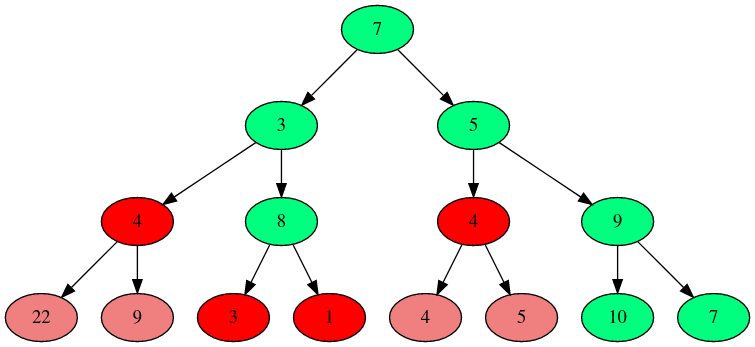
\includegraphics[width=\linewidth]{ilustracije/beam_search_primer.png}
    \caption{Izvršavanje \textit{BS} algoritma nad stablom za širinu pretrage $w = 2$}
    \label{fig:beam_search}
\end{figure}

Pošto se na svakom nivou stabla zadržava samo $w$ čvorova, a prethodno posećeni čvorovi se ne pamte, memorijska složenost ovog algoritma pretrage je $O(w)$, tj. ne zavisi od veličine stabla. Međutim, problem u ovom pristupu je to što će samo $w$ putanja biti u potpunosti (ukoliko su one konačne težine) istraženo, dok su sve ostale putanje odbačene. U kontekstu simboličkog izvršavanja, ovo bi dovelo do gubitka saglasnosti analize. Da bi se ovaj problem rešio, potrebno je izvršiti modifikaciju algoritma, koja je data u vidu \textit{Beam Stack Search} algoritma pretrage.

\subsection{\textit{Beam Stack Search} algoritam pretrage}

Algoritam \textit{Beam Stack Search}, nadalje \textit{BSS}, prvi put je opisan u radu \cite{BeamStackSearch-10.5555/3037062.3037074} i predstavlja nadogradnju osnovnog \textit{Beam Search} algoritma koja rešava prethodni problem odbacivanja potencijalno važnih putanja izvršavanja, ali po cenu povećane memorijske složenosti. Naime, osnovna ideja \textit{BSS} algoritma je u tome da se, umesto odbacivanja, neposećena stanja čuvaju za kasniju obradu u posebno uređenoj stek strukturi. Stek je uređen po nivoima - čvorovi na proizvoljnom nivou stabla koji su razmatrani, ali ne i izabrani za obradu, se postavljaju kao jedan nivo čvorova na steku. U trenutku kada bi standardna \textit{Beam Search} pretraga stigla do kraja stabla, sa vrha steka se uzima jedan nivo čvorova i nastavlja se sa pretragom. Algoritam je prikazan pseudokodom \ref{alg:tree_beam_stack_search}.

\begin{algorithm}
    \begin{algorithmic}[1]
            \Procedure{BSS}{Tree t, Int w}
                \State Vec<Node> currentLevel = \{t.root()\}
                \State Vec<Node> nextLevel = \{\}
                \State Stack<Vec<Node>{>} beamStack = \{\}
                \While {not currentLevel.empty()}
                    \For {Node n in currentLevel}
                        \State visit(n)
                        \State nextLevel.append(t.adjacent(n))
                    \EndFor
                    \State nextLevel.sort()
                    \State Int beamWidth = min(nextLevel.size(), w)
                    \State currentLevel = nextLevel[0 : beamWidth]
                    \If {beamWidth != nextLevel.size()}
                        \State beamStack.push(nextLevel[beamWidth : nextLevel.size()])
                    \EndIf
                    \State nextLevel.clear()
                    \If {currentLevel.empty() and not beamStack.empty()}
                        \State currentLevel = beamStack.top()
                        \State beamStack.pop()
                    \EndIf
                \EndWhile
            \EndProcedure
    \end{algorithmic}
    \caption{Tree Beam Stack Search}
    \label{alg:tree_beam_stack_search}
\end{algorithm}

Upotreba steka sa neposećenim čvorovima garantuje da će svi čvorovi stabla u nekom trenutku biti posećeni, ali njegovo održavanje zahteva dodatnu memoriju u odnosu na klasičan \textit{Beam Search} algoritam. Ukoliko pretpostavimo da je stablo nad kojem se algoritam izvršava binarno, što i jeste validna pretpostavka za osnovni slučaj simboličkog stabla izvršavanja, može se pokazati da je memorijska složenost algoritma ograničena sa dubinom stabla i zadatim parametrom širine pretrage $w$.

\begin{lemma}
Ukoliko se algoritam \textit{Beam Stack Search} primenjuje nad binarnim stablom, memorijska složenost algoritma je $O(dw)$, gde $d$ predstavlja dubinu stabla, a $w$ je zadati parametar širine pretrage.
\end{lemma}

\begin{proof}
Za dokaz je dovoljno pokazati da je (1) veličina svakog nivoa čvorova na steku najviše $w$ i (2) na steku je u svakom trenutku najviše $d$ nivoa čvorova.
\begin{enumerate}
    \item Posmatrajmo skup izabranih čvorova u $i$-toj iteraciji algoritma \ref{alg:tree_beam_stack_search}, u oznaci $currentLevel$. Pre ulaska u petlju, ovaj skup sadrži samo koren stabla, te je njegova kardinalnost jednaka $card(currentLevel) = 1$. U $i-toj$ iteraciji petlje, skup čvorova $currentLevel$ se ažurira tako što se od njima susednih čvorova, u oznaci $nextLevel$, bira $min(w, card(nextLevel))$ njih. Prema tome, važi da je $card(currentLevel) \leq w$ u svakoj iteraciji petlje. Usled uslova da je stablo binarno, dodatno važi i $card(nextLevel) \leq 2 \cdot card(currentLevel) \leq 2w$. Pošto se na stek dodaju skupovi čvorova veličine $card(nextLevel) - w$, iz prethodnog važi da će se na steku u svakom trenutku nalaziti samo skupovi čvorova veličine manje ili jednake od $w$.

    \item Dovoljno je primetiti da nivoi na steku, počev od njegovor vrha, odgovaraju strogo opadajućem redosledu nivoa u stablu, gde najmanji nivo ima koren stabla. Naime, svakim ponovnim pokretanjem pretrage od nekog nivoa na steku se taj nivo skida sa steka, a dalja pretraga do ponovnog pokretanja od nekog nivoa sa steka teče strogo niz stablo, pa sledi da je nivo koji odgovara svakom skupu čvorova koji se dodaje na stek strogo manji od onog koji je prethodno izbačen sa steka, kao i od onog koji je prethodno dodat na stek. Pošto stablo ima najviše $d$ nivoa, sledi da se na steku u svakom trenutku može naći najviše $d$ nivoa čvorova.
\end{enumerate}
\end{proof}

Ovako ograničena memorijska složenost sprečava prebrzo zauzeće memorije kao što je to slučaj kod klasičnog $BFS$ algoritma, ali pritom zadržava mogućnost šireg prostora pretrage i istovremenog praćenja više potencijalno zanimljivih putanja pomoću podesivog parametra širine pretrage $w$. Zapravo, za vrednost parametra $w = 1$, algoritam bi se ponašao kao $DFS$ algoritam pretrage, pri čemu se u svakom koraku bira bolji čvor za nastavak pretrage, dok bi se za dovoljno veliko $w$, vrednosti veće ili jednake širini celokupnog stabla, ponašao kao $BFS$ algoritam. Dodatno, izbor čvorova za posetu prema nekoj izabranoj meri kvaliteta omogućava brži pronalazak kvalitetnih putanja, što bi u kontekstu simboličkog izvršavanja moglo da podrazumeva putanje čije izvršavanje osigurava veliki stepen pokrivenosti koda.

\section{Implementacija u okviru alata za simboličko izvršavanje KLEE}

U projektu koji implementira koncepte iz ovog rada \cite{Projekat} klasa \emph{BeamSearcher} predstavlja specijalizovanu implementaciju klase \emph{Searcher} koja upravlja pretragom stanja primenom modifikovanog
$BSS$ algoritma. Bazna klasa Searcher, koja je apstraktna i implementirana u KLEE alatu,
definiše strategije ili heuristike za selekciju stanja koja će biti dalje istražena.

Klasa BeamSearcher nasleđuje ovu baznu klasu i preopterećuje njene čisto virtualne metode:
\begin{itemize}
    \item \textbf{selectState:} Ova metoda bira jedno stanje za dalje istraživanje. U kontekstu $BSS$ algoritma, bira se prvo stanje u trenutnom sloju.

    \item \textbf{update:} Ova metoda obaveštava pretraživač o novim ili uklonjenim stanjima. Koristi se za ažuriranje slojeva pretrage nakon što su stanja razgranata ili uklonjena.

    \item \textbf{empty} Ova metoda proverava da li su sva stanja istražena, tj. da li pretraživač više nema stanja za istraživanje.
\end{itemize}

\subsection{Modifikacija implementacije algoritma}

U implementaciji klase uvedena je modifikacija algoritma u odnosu na pređašnje opisani $BSS$: parametar \emph{beamStackSwapLimit}, koji je uveden kako bi se izbeglo zaglavljivanje u lokalnim maksimumima tokom pretrage. Ovaj parametar omogućava pretraživaču da, nakon određenog broja iteracija u kojima nije pronađeno novo pokrivanje (\emph{statesSinceLastCoveredNew}), vrati pretragu na početak steka, tj. na ranija stanja umesto da nastavlja sa trenutnog nivoa. Kada je vrednost parametra \emph{beamStackSwapLimit} postavljena na 0, algoritam se ponaša kao klasičan $BFS$.


Specifično, ako \emph{currentLayer} postane prazan, a broj iteracija bez novog pokrivanja premaši \emph{beamStackSwapLimit}, pretraživač će zameniti trenutni sloj sa slojem iz \emph{unvisitedStack}, uzimajući stanja iz ranijih faza pretrage. Na taj način, pretraga može da se vrati na prethodna stanja koja su možda bliža rešenju, čime se povećava šansa za izlazak iz lokalnog maksimuma.

Iako ova modifikacija može povećati memorijske zahteve (gubeći garanciju složenosti od \(O(dw)\)), eksperimentalno se pokazalo da nema značajan negativan uticaj na performanse algoritma, dok istovremeno povećava njegovu robusnost u situacijama sa kompleksnim pretraživačkim prostorima.

\subsection{Metrika}

Koristi se metrika za izbor čvorova koja je zasnovana na istoj strategiji kao i podrazumevani \emph{nurs
} (\emph{Non-Uniform Random Search}) algoritam. Ova metrika kombinuje dve komponente:

\begin{enumerate}
\item Minimalna udaljenost do najbliže nepokrivene instrukcije u grafu kontrole toka.
\item Broj instrukcija izvršenih od poslednje pokrivene nove grane.
\end{enumerate}

Algoritam maksimizuje pokrivenosti koda tako što bira stanja koja će se dalje istraživati biranjem novih, do tada nepokrivenih delova programa. Pošto manja vrednost za obe metrike daje veći prioritet stanju, one se invertuju kako bi se postigao željeni efekat.

\subsection{Pokretanje Algoritma u okviru alata KLEE}

KLEE omogućava korisnicima da prilagode način pretrage kroz nekoliko različitih opcija. Za korišćenje BeamSearcher algoritma, dve ključne opcije su:
\begin{enumerate}
    \item \textbf{beam-width}: Ova opcija postavlja širinu pretrage, što znači broj stanja koja se zadržavaju za dalje istraživanje u svakom sloju pretrage. Širina pretrage određuje koliko različitih grana se istražuje u jednom trenutku. Podrazumevana vrednost za ovu opciju je 256.
    \item \textbf{beam-stack-swap-limit}:  Ova opcija određuje broj stanja koja će biti posećena u nizu bez pokrivanja nove instrukcije pre nego što se pretraga vrati na početak steka. Ako je postavljena na 0, pretraga će se ponašati kao klasična $BFS$. Podrazumevana vrednost je 1.000.000.
\end{enumerate}

Da biste pokrenuli KLEE koristeći \emph{BeamSearcher} sa specifičnim vrednostima za \emph{beam-width} i \emph{beam-stack-swap-limit}, možete koristiti sledeću komandu:

\begin{verbatim}
klee --searcher=beam \
    --beam-width=128 \
    --beam-stack-swap-limit=500000 \
    /putanja/do/programa.bc
\end{verbatim}

Ova komanda pokreće KLEE sa BeamSearcher algoritmom, postavlja širinu beam pretrage na 128, i ograničava broj iteracija bez pokrivanja nove instrukcije na 500.000 pre nego što pretraga pređe na ranija stanja.


\section{Eksperimentalna evaluacija algoritma}


\section{Zaključak}

\addcontentsline{toc}{section}{Literatura}
\appendix
\bibliography{literatura} 
\bibliographystyle{plain}

\end{document}
